\chapter{Implementation}
Dieses Kapitel beleuchtet einige Gesichtspunkte der Umsetzung. Die Logik, Abgrenzungen, Einhaltung des Konzepts, verwendete Plattformen und Libraries gehören dazu.
\section{Abgrenzung}
Zu Beginn der Realisierung mussten die Ziele abgegrenzt werden. Der Umfang vom definierten Anforderungskatalog und Konzept ist sehr gross. Für die Umsetzung wurden einige Kernelemente ausgesucht.
\subsection{Ziele - siot.net Gateway Library}
- Die siot.net Gateway Library als Prototypen realisiert werden. \\
- Mindestens die Verbindung zum siot.net aufnehmen können.\\
- Sensoren nach dem siot.net Messagedesign (vgl. \cite{siot:cobo} manifestieren.\\
- Daten an die \gls{IoT}-Cloud im richtigen Format senden.\\
- In einer Applikation integriert werden.
\subsection{Ziele - siot.net Sensorcenter}
- Als Demoapplikation für die Gateway Library umsetzen.\\
- Für Smartphone und Smartwatch lauffähig.
\section{Implementation - siot.net Gateway Library}
Die Umsetzung erfolgte grösstenteils nach dem konzeptionierten Domänenmodell (siehe Abbildung 9.2). Nicht alle Funktionen wurden realisiert. LocationService und der ReceivedMessageManager sind nicht erfolgreich funktional umgesetzt worden. Der LocationService wurde ausgelassen, da dieser sich sehr dem SensorService ähnelt. Beim ReceivedMessageManager wurde bei der Umsetzung festgestellt, dass das Konzept nicht konsistent den Nutzen abdeckt. Dieser Manager muss überarbeitet und womöglich neu konzipiert werden.
\subsection{Klassendiagramm}
Auf der folgenden Seite ist (auf Abbildung 10.1) das Klassendiagramm der siot.net Gateway Library zu sehen. Die realisierten Klassen, sowie die entworfenen, jedoch nicht funktional umgesetzten Objekte (weisser Hintergrund), sind auf dieser Grafik visualisiert.
\newpage
\begin{landscape}
\begin{figure}[H]
  \centering
  \includegraphics[scale=0.1]{98_Bilder/10_Implementation/KlassendiagrammSiotNetGatewayLibrary}
  \caption[siot.net Gateway Library Klassendiagramm]{Die Gesamtübersicht aller Klassen der siot.net Gateway Library}
\end{figure}
\end{landscape}
\newpage
\subsection{Logik}
Einige interessante Logikaspekte sind in den \textit{SiotNetGatewayManager} Klassen enthalten. Mit Hilfe des Mobile Managers benötigt es für den Verbindungsaufbau zum \gls{MQTT} Broker nur die siot.net Lizenz. Beim ausführen der \textit{connectToSiotNet(Lizenz)} Methode, wird per \gls{REST}-\gls{API} ein Authentifikationstoken angefordert. Um ein solches zu erhalten, wird ein \gls{HTTP} GET Request abgesetzt, welches eine Bestätigung oder Zurückweisung im \gls{JSON}-Format retourniert. Diese ist in der \textit{RestClient} Klasse implementiert. Die Antwort wird auf den Messagetyp \textit{SiotUrl} geparst. Die Broker URL wird aus der positiven Bestätigung gelesen.

Mit der aktuell erhaltenen Broker URL kann die Kopplung zum \gls{MQTT} Broker starten. Für diese Angelegenheit dient die \textit{MQTTClient} Klasse. Der \textit{MQTTClient} Objekttyp ist eine, nach dem Prinzip des Singleton-Entwurfsmuster (vgl. \cite{gof:design_patterns} Chapter 3. Creational Patterns) implementierte, Klasse. Von der Library soll immer nur ein Objekt der Klasse \textit{MQTTClient} bestehen, da dieser die Verbindung zum Broker verwaltet, also die Meldungen sendet und auch empfängt. Das Empfangen von Nachrichten durch mehrere Clients würde redundante Daten schaffen, wenn mehrere Subscriber auf dieselbe Topic hören. Desweitern würde die Netzwerkverbindung und Stromversorgung unnötig belastet werden. Der Singleton eignet sich ideal, diese Probleme zu beseitigen.

Um ein Objekt aus der \textit{SiotNetGatewayManagerWear} Fabrikklasse (Entwurfsmuster Fabrikmethode, vgl. \cite{gof:design_patterns} Chapter 3. Creational Patterns) zu erzeugen, ist zwingend eine gültige Verbindung zum Smartphone nötig. Diese wird in Form von einer \textit{GoogleApiClient} Instanz und der NodeId des Smartphone verlangt. Beim instanziieren muss die Überprüfung der gültigen Kopplung von Mobile und Wearable bestanden werden. Im Konzept wurde eine Überprüfung nicht in Erwägung gezogen. Die vorhandene Verbindung ist essentiell für die Funktionsweise der Smartwatch-App.

Nach erfolgreichem kreieren der Manager Elemente, können die Sensoren aktiviert werden. Die \textit{SensorenService} Klassen sind auch nach der Fabrikmethode konzipiert und implementiert. Sensoren müssen bei der ersten Aktivierung beim siot.net manifestiert werden. Eine Besonderheit dabei ist, dass jeder physische Sensorwert einzeln angemeldet wird. Dies muss in der Applikation verwaltet werden. Für dies wurde eine zweidimensionale Hashmap entworfen und verwendet. Die erste Dimension enthält den Schlüssel des Sensortypes, welcher eindeutig vom System vergeben ist und mit der zweiten Hashmap verknüpft ist. Die zweite beinhaltet den Namen des Messwertes (z.B. X-Achse) als Schlüssel und die siot.net \gls{GUID} des physischen Sensorswertes. Beim stoppen und starten eines Sensors kann die \gls{GUID} anhand vorhandener Informationen (Sensortyp und Messwertenamen) und der Zuweisung in der Hashmap evaluiert werden. Die \gls{GUID} wird, für das Manifestieren des Sensors, durch die \textit{GUIDUtil} Klasse generiert. Jeder Senorservice ist auch für das Versenden der Messwerte zuständig. Der MobileService sendet diese direkt per \gls{MQTT} an den Broker. Der WearService sendet eine Message\gls{API} Nachricht, im Format des Messagetyps \textit{WearableData}, an das Smartphone. Beim Konzept wurde definiert, dass über die Manager versendet wird. Dies wurde umkonzeptioniert, so dass die \textit{SensorService} den Manager nicht kennen müssen. Es wurde eine nicht notwendige Abhängigkeit aufgelöst.

Die \textit{ReceivedMessageManager} Klasse wurde während der Entwicklung gestoppt, da erkennt wurde, dass das Konzept für die Bedürfnisse nicht genügend tief konstruiert war. Bei einer Umsetzung, wie in Abschnitt 9.1 beschrieben, wäre dies zu Dateninkonsistenzen und Redundanzen gekommen. Erste Ansätze wurden betrachtet. Eine Überlegung daraus war ein Konstrukt aus der Kombination vom Singleton und dem Observer-Pattern zu formen. Der Stopp dieses Konstruktes führt dazu, dass die Bibliothek die Aktoren noch nicht mit Daten beliefern kann.
\section{Implementation - siot.net Sensorcenter}
Vom Domänendiagramm (siehe Abbildung 9.8) wurde leicht abgewichen. Die \textit{MessageReceiver} Klasse wurde für Android und Android Wear als lokale, innere Klasse der Activity Klasse realisiert. Dies hat den Vorteil, die Objekte der äusseren Klasse zu kennen und selbst nicht nach Aussen sichtbar ist. Das Kernelement dieser Applikation ist das Kommunikationsverhalten von Smartwatch und Smartphone. Weitere Informationen dazu im Abschnitt Logik.
\newpage
\subsection{Klassendiagramm}
Abbildung 10.2 stellt klar, wie kompakt die Entwicklung einer externen Applikation sein kann. Sie zeigt alle Klassen der Android und Android Wear App.
\begin{figure}[H]
  \centering
  \includegraphics[scale=0.18]{98_Bilder/10_Implementation/KlassendiagrammSiotNetSensorcenter}
  \caption[siot.net Sensorcenter Klassendiagramm]{Klassendiagramme für das Android und Android Wear Sensorcenter}
\end{figure}
\subsection{Logik}
Diese Applikationen verwenden die siot.net Gateway Library und deren Logik. Erweiterte logische Elemente gibt es für die Handhabung der Verbindung von Smartwatch und Smartphone und das Verhalten der grafischen Oberfläche.

Die Kommunikation wurde, wie im Konzept definiert, umgesetzt. Wenn eine Smartwatch die Applikation startet, wird per \textit{GoogleApiClient} ein Kommunikationstunnel zum Smartphone hergestellt. Dabei wird gleich die erste Nachricht via Message\gls{API} versendet, mit der Aufforderung, das Sensorcenter auf dem Smartphone zu öffnen. Die Klasse \textit{WearListenerService} empfängt alle Messages, welche durch diesen eröffneten Kanal gesendet werden. Auch wenn die App noch nicht läuft, kann die Nachricht verarbeitet werden. Das ist möglich, weil der Listener als Service im Android System registriert wird. Zu erreichen ist dies durch einen Eintrag im AndroidManifest.

Nach dem die Applikation läuft, kann die Verbindung zu siot.net aufgebaut werden. Für die Wear App ist es notwendig, dass die Mobile App auch läuft. Der Aufbau der Kommunikationsleitung erfolgt, wie auf Abbildung 9.6 (Smartphone) und Abbildung 9.7 (Smartwatch) illustriert. Die Android Wear Anwendung sendet hier eine CONNECT Message\gls{API} Nachricht ans Android Gerät. Wenn die Leitung zu siot.net noch nicht steht, wird diese aufgebaut und eine positive Antwort an die Uhr verschickt. Nach erfolgtem Verbindungsaufbau, werden die Ein- und Ausschalter der Sensoren freigegeben. Es werden nur jene angezeigt, welche für das Gerät relevant sind.

Beim Abmelden verhaltet es sich ein wenig differenziert. Die Smartwatch meldet sich nur beim Smartphone als Sensorcenter ab. Es geschehen keine weiteren Aktionen. Durch die Mobile App wird die Verbindung zu siot.net instandgehalten. Dies wird so gehandhabt, da das Sensorcenter des Smartphones in der Zwischenzeit auch zu Verwendung kommen könnte. Das Smartphone löst beim Abmelden eine DISCONNECT Nachricht, an die verbundene Smartwatch, aus. Es signalisiert, dass keine Verbindung mehr zum siot.net \gls{MQTT} Broker besteht. Das Wearable reagiert umgehend und stoppt die Messungen und zeigt an, dass es nicht mehr verbunden ist.

Messwerte der Uhr können nicht direkt ins Internet verbreitet werden, weshalb das Smartphone diese per Message\gls{API} als WearableData Messagetyp erhält. Diese können nun mit Hilfe der öffentlichen Methode \textit{publishData(topic, data)} der SiotNetGatewayManagerMobile Instanz, an den \gls{MQTT} Broker publiziert werden.

Aufgrund nicht lange ausdauernden Akkus, sind Android Wear Apps für den Betrieb im Hintergrund nicht geeignet. Normalerweise wird die laufende Smartwatch Applikationen beendet, wenn das Display in den Standby-Modus geht. Um bei Verdunklung des Bildschirmes die Arbeit des Sensorcenters nicht zu unterbrechen, muss das Gerät eines der folgenden Funktionen unterstützen: Always-On Screen oder den Ambient Mode. Ersteres lässt die Uhr nie in den Ruhezustand kehren. Das Zweite lässt die Applikation laufen und verfinstert den Touchscreen, um den Akku zu schonen. Um beide Methoden zu aktivieren, muss dies in der \textit{WearSensorPublisherActivity} implementiert werden.
\subsection{MessageAPI Messagetypen}
\begin{table}[H]
\centering
\begin{tabular}{|>{\columncolor[gray]{0.8}}p{3cm}|p{13.5cm}|}
\hline
\textbf{START\_APP}  & Nachricht von Smartwatch zu Smartphone, dass App gestartet werden soll. Wird bei Erfolg quittiert.\\ \hline
\textbf{CONNECT}    & Nachricht von Smartwatch zu Smartphone, dass die Verbindung zu siot.net aufgebaut werden soll. Wird bei Erfolg mit ok oder bei Misserfolg mit einer DISCONNECT Nachricht quittiert.\\ \hline
\textbf{DISCONNECT} & Nachricht von Smartwatch zu Smartphone, dass die Verbindung nicht mehr benötigt wird. Smartphone quittiert mit ok.\newline Nachricht von Smartphone zu Smartwatch, dass die Verbindung zu siot.net geschlossen wird. Smartwatch quittiert mit ok und schliesst die Verbindung. \\ \hline
\textbf{SEND\_DATA}  & Nachricht von Smartwatch zu Smartphone. Daten werden im \textit{WearableData} Messagetyp der siot.net Gateway Library gesendet. Nachricht wird nicht quittiert. \\ \hline
\end{tabular}
\caption{siot.net Sensorcenter: MessageAPI Messagetypen}
\end{table}
\subsection{Graphical User Interface}
Das \gls{GUI} beider Softwareartefakte ist sehr simpel und geradlinig gehalten, da es hauptsächlich zu Demonstrationszwecke dienen soll.
\begin{figure}[H]
  \centering
  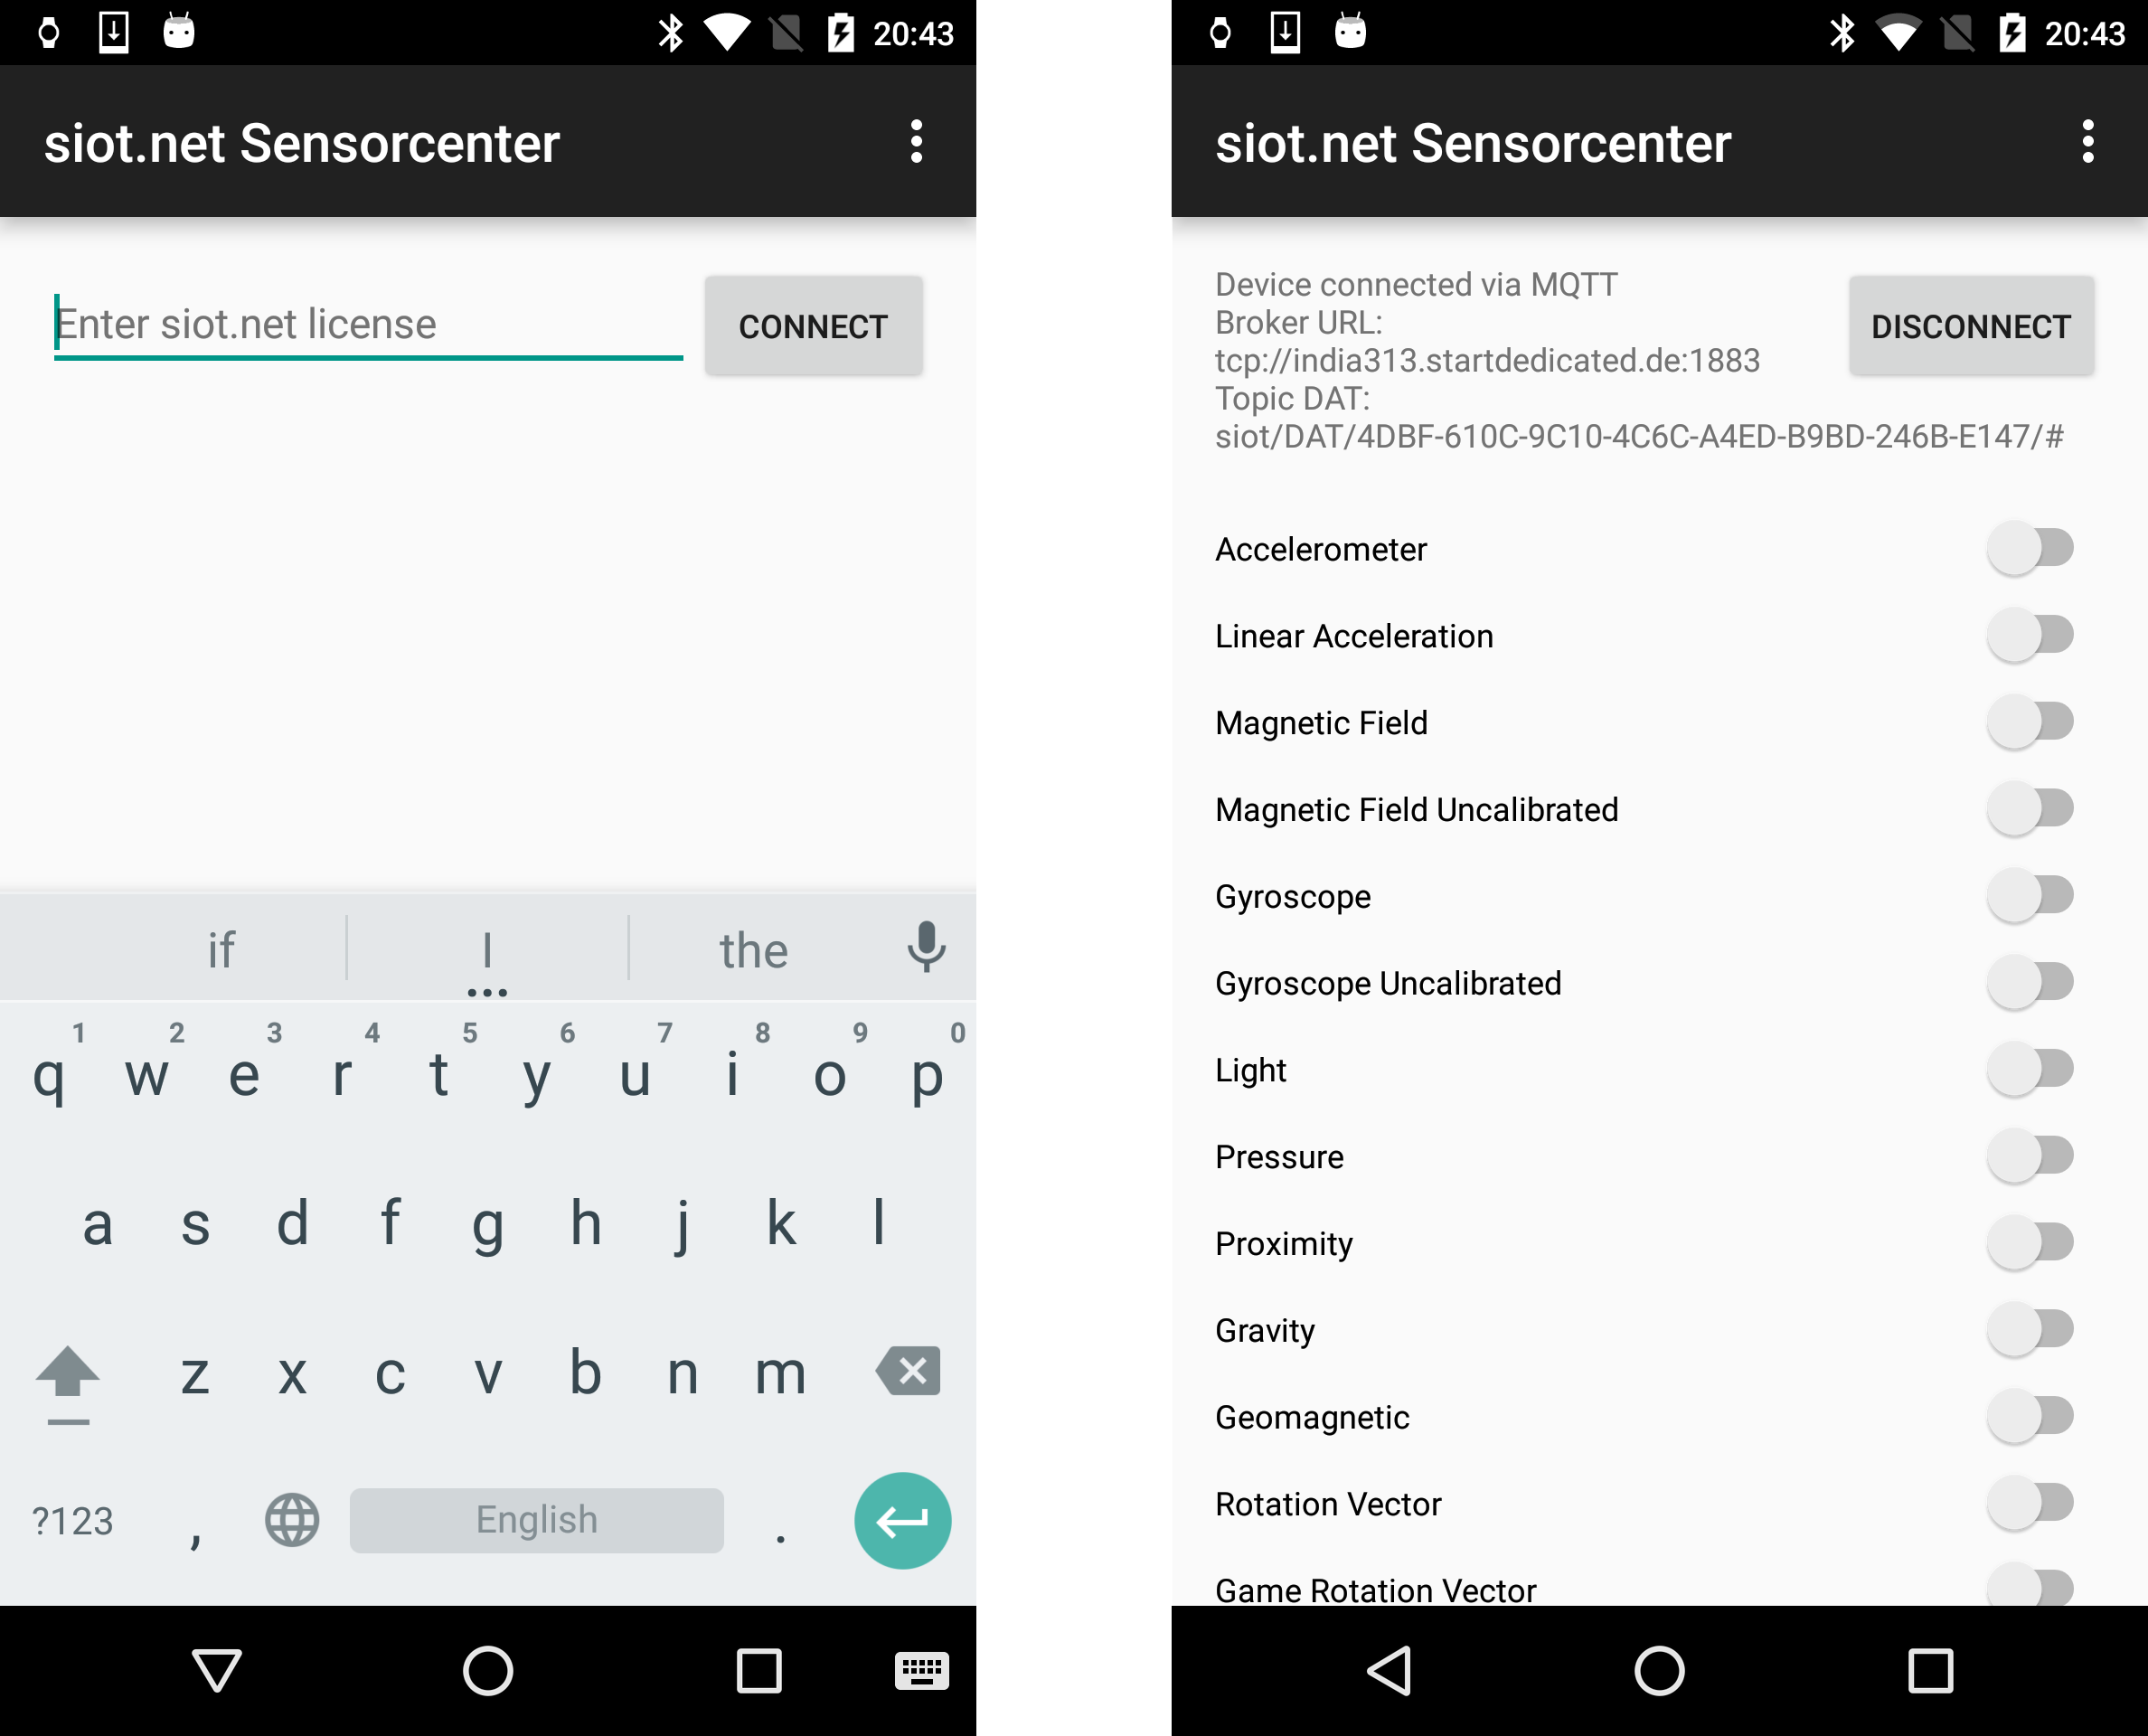
\includegraphics[scale=0.15]{98_Bilder/10_Implementation/01_Sensorcenter}
  \caption[siot.net Sensorcenter Smartphone Screens]{Die möglichen Ansichten des Sensorcenter eines Smartphones}
\end{figure}
Die Android Mobile App ist eine schlanke, zweisegmentale Ansicht. Oben das Feld mit der Texteingabe oder dem Informationsbereich und dem Knopf. Die Abbildung 10.3 zeigt, dass das untere Teilstück die Schalter für die Sensoren darstellt, wenn der Benutzer eingeloggt ist.\\
Zur Verwendung gekommene \gls{GUI} Elemente sind: Textfeld, Informationstextfeld, Knopf und mehrere Ein- und Ausschalter. Für Benachrichtigungen werden Toast am unteren Teil des Bildschrims eingeblendet.
\begin{figure}[H]
  \centering
  \includegraphics[scale=0.5]{98_Bilder/10_Implementation/02_Sensorcenter}
  \caption[siot.net Sensorcenter Smartwatch Screens]{GUI Elemente des Smartwatch Sensorcenters}
\end{figure}
Das \gls{GUI} der Smartwatch Anwendung ist noch minimalistischer, dies visualisiert die Abbildung 10.4. Der Touchscreen der Uhr ist eher klein, infolge dessen werden nur die wichtigsten Informationen angezeigt. Aus diesem Grund wir nur ein Knopf und die Ein- und Ausschalter für die einzelnen Sensoren eingeblendet. Die grafische Benutzeroberfläche ist so implementiert, dass es im Always-On Display Modus, sowie Ambient Mode funktioniert.\\
Ein Aspekt, der bei der Realisierung des \gls{GUI}s beachtet werden musste, waren die unterschiedlichen Formen, sowie den Spezialitäten wie ein unförmiges Display. Die zwei Test-Smartwatch waren nicht vom gleichen Typ. Die LG G Watch hat ein rechteckiges Display, die Motorola Moto 360 ein Rundes mit einem abgeflachten Ende.

\section{Plattformen und Libraries}
Für die Entwicklung der Android, Android Wear Bibliothek und App, wurde ausschliesslich Android Studio verwendet. Die Abbildung 10.5 zeigt, dass die Entwicklungsumgebung einige Abhängigkeiten hat. Für die eingesetzten Sprachen Java und XML wurde Android Studio (A) genutzt, welche auf der IntelliJ IDEA Plattform basiert. Es bietet Gradle als flexibles Build-Management-Automatisierungs-Tool. Dies nutzt eine Groovy(B) basierende domänenspezifische Sprache (DSL) zur Beschreibung der zu erstellenden Artefakte. Die benutzten Bibliotheken werden in dieser Beschreibungsdatei erfasst. Libraries können in einem Lokalen Verzeichnis(D) oder in einer globalen Ablage, z.B. jCentral (vgl. \cite{grdl:jcenter})(C), referenziert sein.
\begin{figure}[H]
  \centering
  \includegraphics[scale=0.28]{98_Bilder/10_Implementation/PlattformLibraries}
  \caption[Plattforme, Libraries]{Genutzte technische Elemente und deren Abhängigkeiten}
\end{figure}
\subsection{Google Play Services}
Die Google Play Services sind ein proprietärer Hintergrund Service und eine Applikationsschnittstelle (\gls{API}) für Android Geräte. Die verwendeten Message\gls{API} und GoogleClientApi stammen aus dieser Sammlung.
\subsection{Google Gson}
Diese Bibliothek wird verwendet um die Messagetypen von einem POJO in ein \gls{JSON} zu konvertieren.
\subsection{Eclipse Paho MQTT}
Das Paho Projekt (vgl. \cite{eclp:paho}) von Eclipse, liefert die Client Implementation des \gls{MQTT} Nachrichtenprotokoll. Für die Implementation des Nachrichtenaustausches zu siot.net, kommt diese zum Einsatz.

\section{Dokumentation}
Der gesamte Quelltext ist dokumentiert und als JavaDoc auf dem digitalen Anhangsmedium abgelegt. Zusätzlich ist ein Entwicklerhandbuch geschrieben worden, welches im Anhang zu finden ist.
